%%=============================================================================
%% Audio- en videospelers
%%=============================================================================

\chapter{Audio- en videospelers}%
\label{ch:audioenvideo}

In dit hoofdstuk worden de audio- en videomogelijkheden van native en cross-platform vergeleken met elkaar. 
Met de resultaten kan dan een gepaste conclusie worden gevormd.

\section{Native}
\subsubsection{Wat is er nodig}
Om audio en video af te spelen binnen een applicatie wordt gebruik gemaakt van het MediaPlayer 
framework en de VideoView klasse. Deze stellen ons in staat om gemakkelijk audio en video af te spelen binnen 
onze applicatie. Er kunnen zowel lokale files als streams van het internet worden gebruikt.

\subsubsection{Uitvoering}

\paragraph{1. Permissions toevoegen}
Indien het scherm van de applicatie niet mag uitvallen als er 
audio of video afspeelt, dan moet volgende permission worden toegevoegd aan het 
\textbf{AndroidManifest.xml} bestand.
\begin{minted}{xml}
<uses-permission android:name="android.permission.WAKE_LOCK" />
\end{minted}

\paragraph{2. Variabelen initialiseren, vinden en linken}
Om de MediaPlayer en VideoView te gebruiken, moeten er eerst variabelen voor 
worden aangemaakt. Daarna moeten de variabelen gelinkt worden met het juiste element in de layout.
\begin{minted}{kotlin}
private var mediaPlayer: MediaPlayer? = null
private var videoView: VideoView? = null

override fun onCreate(savedInstanceState: Bundle?) {
    super.onCreate(savedInstanceState)
    setContentView(R.layout.activity_main)
    // R.raw.sample is een audio file in de raw folder
    mediaPlayer = MediaPlayer.create(this, R.raw.sample)
    videoView = findViewById(R.id.videoView)
    videoView?.setVideoPath("Video URL")
}
\end{minted}

\paragraph{3. Audio en video afspelen, pauzeren en stoppen}
Om audio en video af te spelen, pauzeren en stoppen worden de 
\textbf{start()}, \textbf{pause()} en \textbf{stop()} methodes van de
MediaPlayer en de VideoView gebruikt.
\begin{minted}{kotlin}
// Audio
mediaPlayer?.start()
mediaPlayer?.pause()
mediaPlayer?.stop()

// Video
videoView?.start()
videoView?.pause()
videoView?.stopPlayback()
\end{minted}
Deze worden dan gekoppeld aan een knop in de layout om de audio en video
af te spelen, pauzeren en stoppen.
\begin{minted}{kotlin}
val playButton = findViewById<Button>(R.id.playButton)
playButton.setOnClickListener {
    mediaPlayer?.start()
    videoView?.start()
}
\end{minted}

\paragraph{4. Applicatie maken}
Nu wordt de applicatie aangemaakt om audio en video af te spelen, pauzeren en
stoppen. Deze bestaat uit een layout met telkens drie \textbf{Button} componenten 
voor het starten, pauzeren en stoppen voor zowel de audio en video. De video 
wordt afgespeeld in een \textbf{VideoView} component. De audio wordt afgespeeld
met een \textbf{MediaPlayer} object.
\begin{figure}[H]
    \centering
    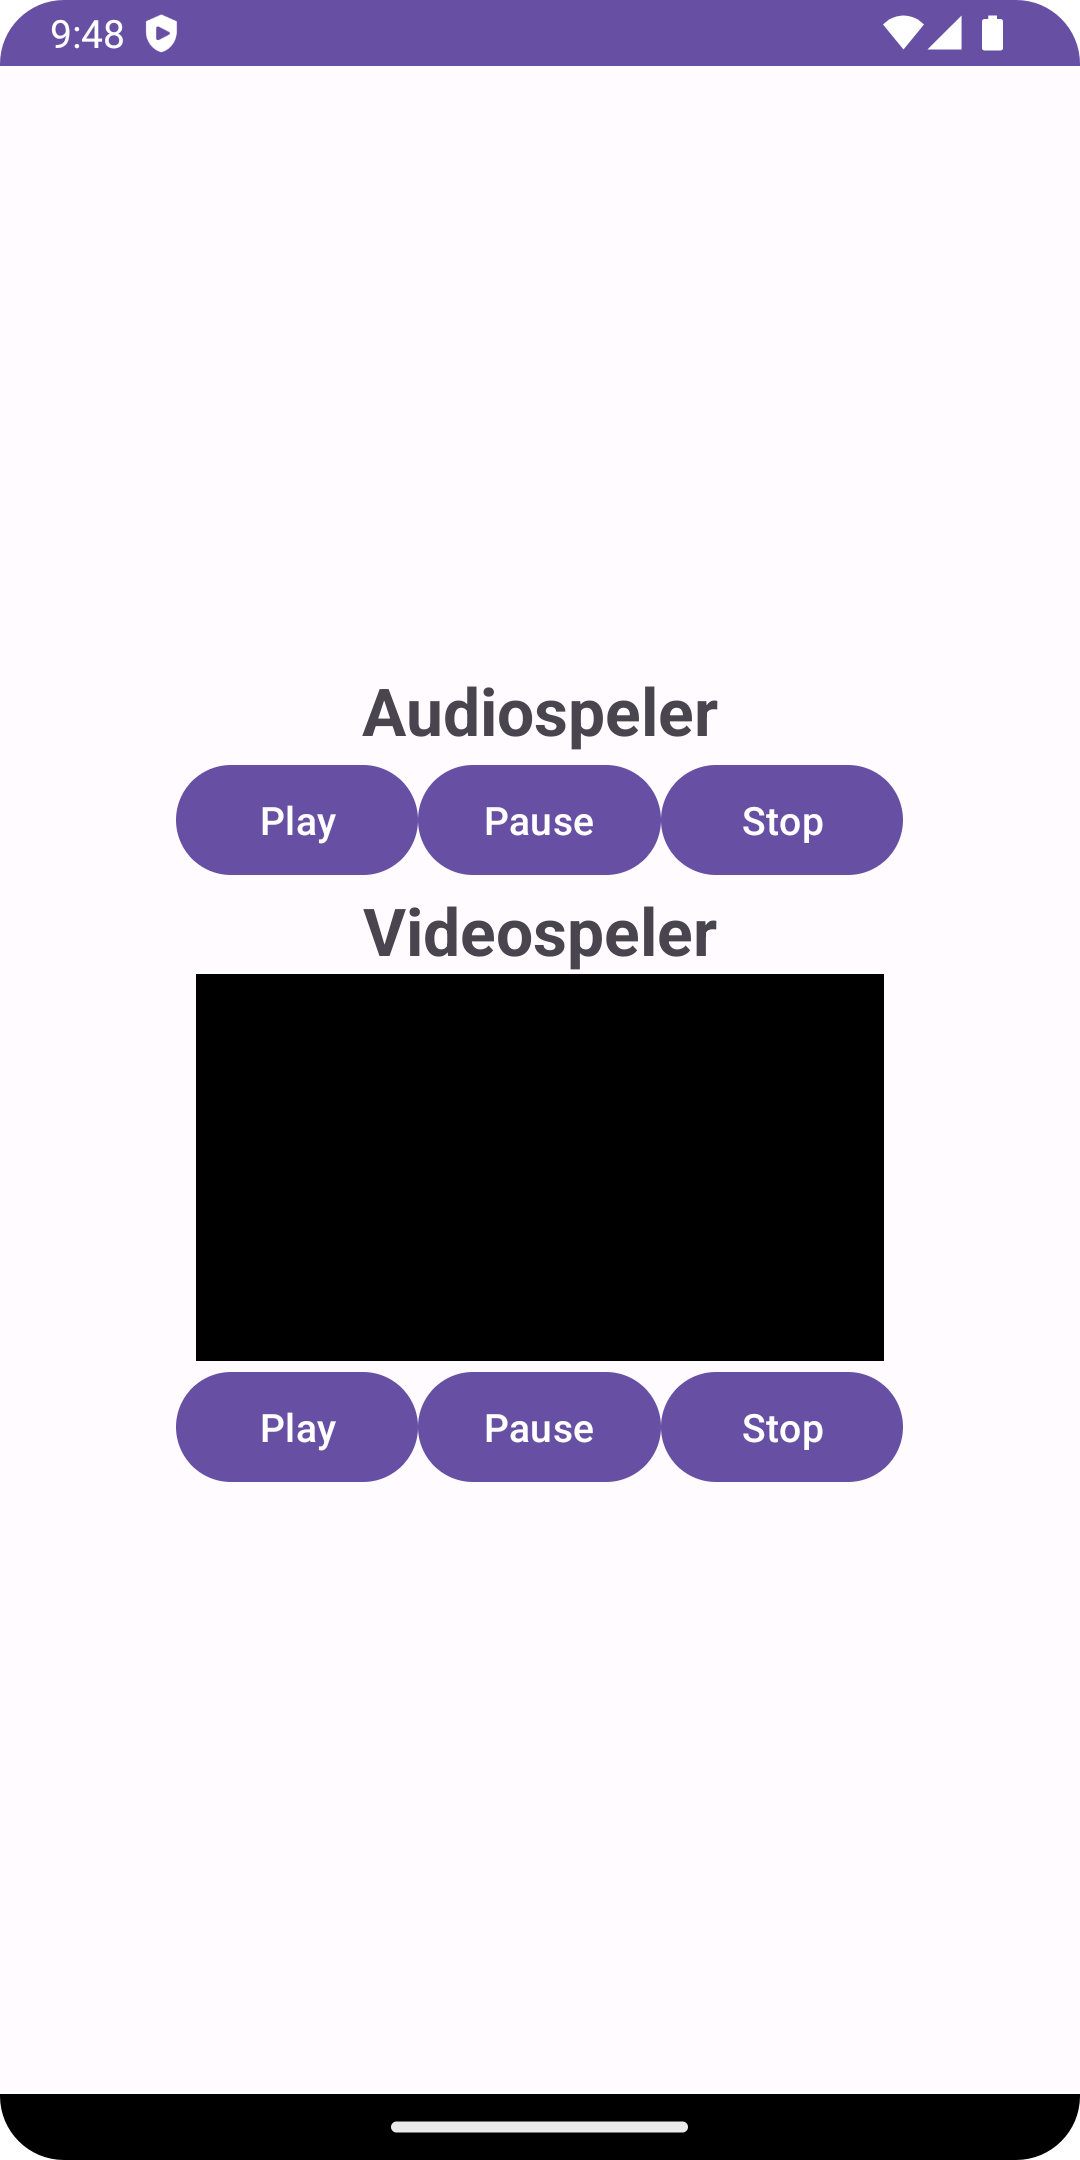
\includegraphics[height=0.5\textheight]{media_layoutnative.png}
    \caption{Layout van applicatie voor het afspelen van audio en video bij Android.}
\end{figure}






\subsubsection{Ontwikkeltijd}

Er moest enkel een variabel aangemaakt worden, deze linken aan de juiste elementen
in de layout en dan de juiste methodes oproepen. Dit was zeer simpel en snel te
implementeren. De applicatie was daardoor ook zeer snel gemaakt. Het duurde ongeveer 45 minuten 
om de functionaliteiten te implementeren en de applicatie te maken.




\subsubsection{Performantie}

\paragraph{Tijdsduur}
Bij het afspelen van audio of video is er niet echt een meting om te doen. 
De audio of video dat afspeelt is ofwel spelend ofwel niet spelend.
Daarom wordt er enkel gekeken naar het CPU en geheugen gebruik tijdens 
het afspelen van audio en video.

\paragraph{CPU \& geheugen}
\begin{figure}[H]
    \centering
    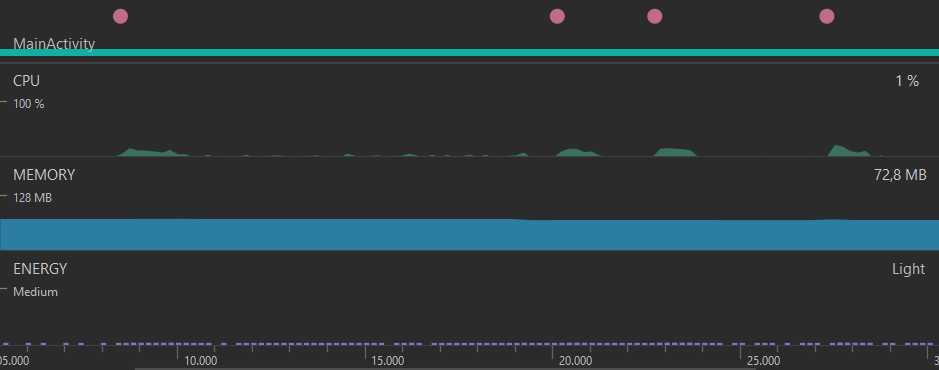
\includegraphics[height=0.25\textheight]{mediaPerformantieNative.png}
    \caption{Overzicht CPU en geheugen gebruik tijdens het afspelen van audie en video bij Android.}
\end{figure}
De eerste twee klik events zijn voor het starten en pauzeren van de video. Op de grafiek 
is te zien dat het CPU gebruik stijgt tot 17\% en daarna afwzakt naar een wisselend gebruik 
van 0 - 7\%. Bij het pauzeren van de video stijgt het CPU gebruik tot 16\% en daarna
zakt het terug naar 0\%. Het geheugen gebruik tijdens het afspelen van de video komt overeen 
met het geheugen gebruik bij het inactief zijn van de applicatie. Er is dus geen verschil in
geheugen gebruik bij het afspelen van de video.
\\\\
De laatste twee klik events zijn voor het starten en pauzeren van de audio. Op de grafiek
is te zien dat het CPU gebruik opnieuw stijgt tot 17\%. In tegenstelling tot de video is 
er geen wisselend CPU gebruik. Het CPU gebruik blijft constant rond 0 - 1\%. Bij het pauzeren
van de audio stijgt het CPU gebruik tot 23\% en zakt daarna terug naar 0\%. En net zoals bij de 
video is er geen verschil in geheugen gebruik bij het afspelen van de audio. Het geheugen gebruik
tijdens het afspelen van de audio komt opnieuw overeen met het geheugen gebruik bij het inactief zijn van
de applicatie.

\subsubsection{Schaalbaarheid}

\paragraph{Complexiteit}
Het implementeren van een audio- en videospeler in Android is zeer simpel. 
Er moet geen extra library of tool worden gebruikt. Er moet enkel een variabel worden aangemaakt
en gelinkt worden aan de juiste elementen in de layout.

\paragraph{Herbruikbaarheid}
Aangezien de code zeer simpel is en er geen extra library of tool wordt gebruikt,
is de code zeer herbruikbaar. De code kan gebruikt worden in elke applicatie of klasse die audio en video
moet afspelen. In verband met de schaling, is het mogelijk om de audio- en videospeler te abstracteren 
en deze dan vanuit één centrale plaats op te schalen. 



\section{Cross-platform}
\subsubsection{Wat is er nodig}
Om audio en video af te spelen binnen een cross-platform applicatie wordt gebruik gemaakt van de
react-native-track-player en react-native-video libraries. Deze stellen ons in staat om gemakkelijk 
audio en video af te spelen binnen onze applicatie. Er kunnen zowel lokale files als streams van 
het internet worden gebruikt.

\subsubsection{Uitvoering}

\paragraph{1. Library toevoegen}
Eerst moeten de libraries aan de root van ons project worden toegevoegd. 
Deze worden toegevoegd met volgende commando's:
\begin{minted}{bash}
npm install --save react-native-track-player
npm install --save react-native-video
\end{minted}

\paragraph{2. Package teruggeven}
Normaal gezien moet de package dan worden toegevoegd aan het 
\textit{android/app/src/} \textit{main/java/com/project/MainApplication.java} bestand.
Maar dit is niet meer nodig bij React Native 0.60+.

\paragraph{3. Audio library initialiseren}
Om de audiospeler te kunnen gebruiken, moet een service bestand worden geregistreerd in de main 
component van de applicatie, meestal is dit het \textit{index.js} bestand.
\begin{minted}{javascript}
import TrackPlayer from 'react-native-track-player';
// AppRegistry.registerComponent(...);
TrackPlayer.registerPlaybackService(() => require('./service.js'));
\end{minted}
Daarna moet er een service worden aangemaakt in een apart \textit{service.js} bestand.
\begin{minted}{javascript}
module.exports = async function() {
    // ...
}
\end{minted}
Tot slot moet de TrackPlayer worden opgezet met de \textbf{setupPlayer()} methode. Deze methode
moet worden aangeroepen voor de \textbf{TrackPlayer} kan worden gebruikt.
\begin{minted}{javascript}
import TrackPlayer from 'react-native-track-player';

await TrackPlayer.setupPlayer()
\end{minted}

\paragraph{4. Audio- en videospeler gebruiken}
\subparagraph{4.1. Audio}
Om de audiospeler te gebruiken moet eerst een \textbf{Track} object worden aangemaakt.
\begin{minted}{javascript}
const track = {
    url: require(''),
    title: 'Title',
    artist: 'Artist',
    artwork: require(''),
    duration: 100
};
\end{minted}
Daarna wordt deze aan het \textbf{TrackPlayer} object toegevoegd.
\begin{minted}{javascript}
await TrackPlayer.add(track);
\end{minted}
Nu is het mogelijk om de audio te starten, pauzeren en stoppen met behulp 
van een aantal \textbf{<Button>} componenten.
\begin{minted}{javascript}
<Button title="Play" onPress={() => TrackPlayer.play()} />
<Button title="Pause" onPress={() => TrackPlayer.pause()} />
<Button title="Stop" onPress={() => TrackPlayer.stop()} />
\end{minted}

\subparagraph{4.2. Video}
Om de videospeler te gebruiken, moet eerst een \textbf{<Video>} component worden aangemaakt.
\begin{minted}{javascript}
<Video source={require('')} />
\end{minted}
Nu is het mogelijk om de video te starten, pauzeren en stoppen met behulp
van een aantal \textbf{<Button>} componenten.
\begin{minted}{javascript}
<Button title="Play" onPress={() => this.video.play()} />
<Button title="Pause" onPress={() => this.video.pause()} />
<Button title="Stop" onPress={() => this.video.stop()} />
\end{minted}

\paragraph{5. Applicatie maken}
Net zoals bij native bestaat de applicatie voor elke audio- en videospeler uit een \textbf{<View>}
component met daarin de \textbf{<Button>} componenten om de audio of video te starten, te pauzeren
of te stoppen. Daarnaast bevat de applicatie ook een \textbf{<View>} component met daarin een
\textbf{<Video>} component voor het afspelen van de video.
\begin{figure}[H]
    \centering
    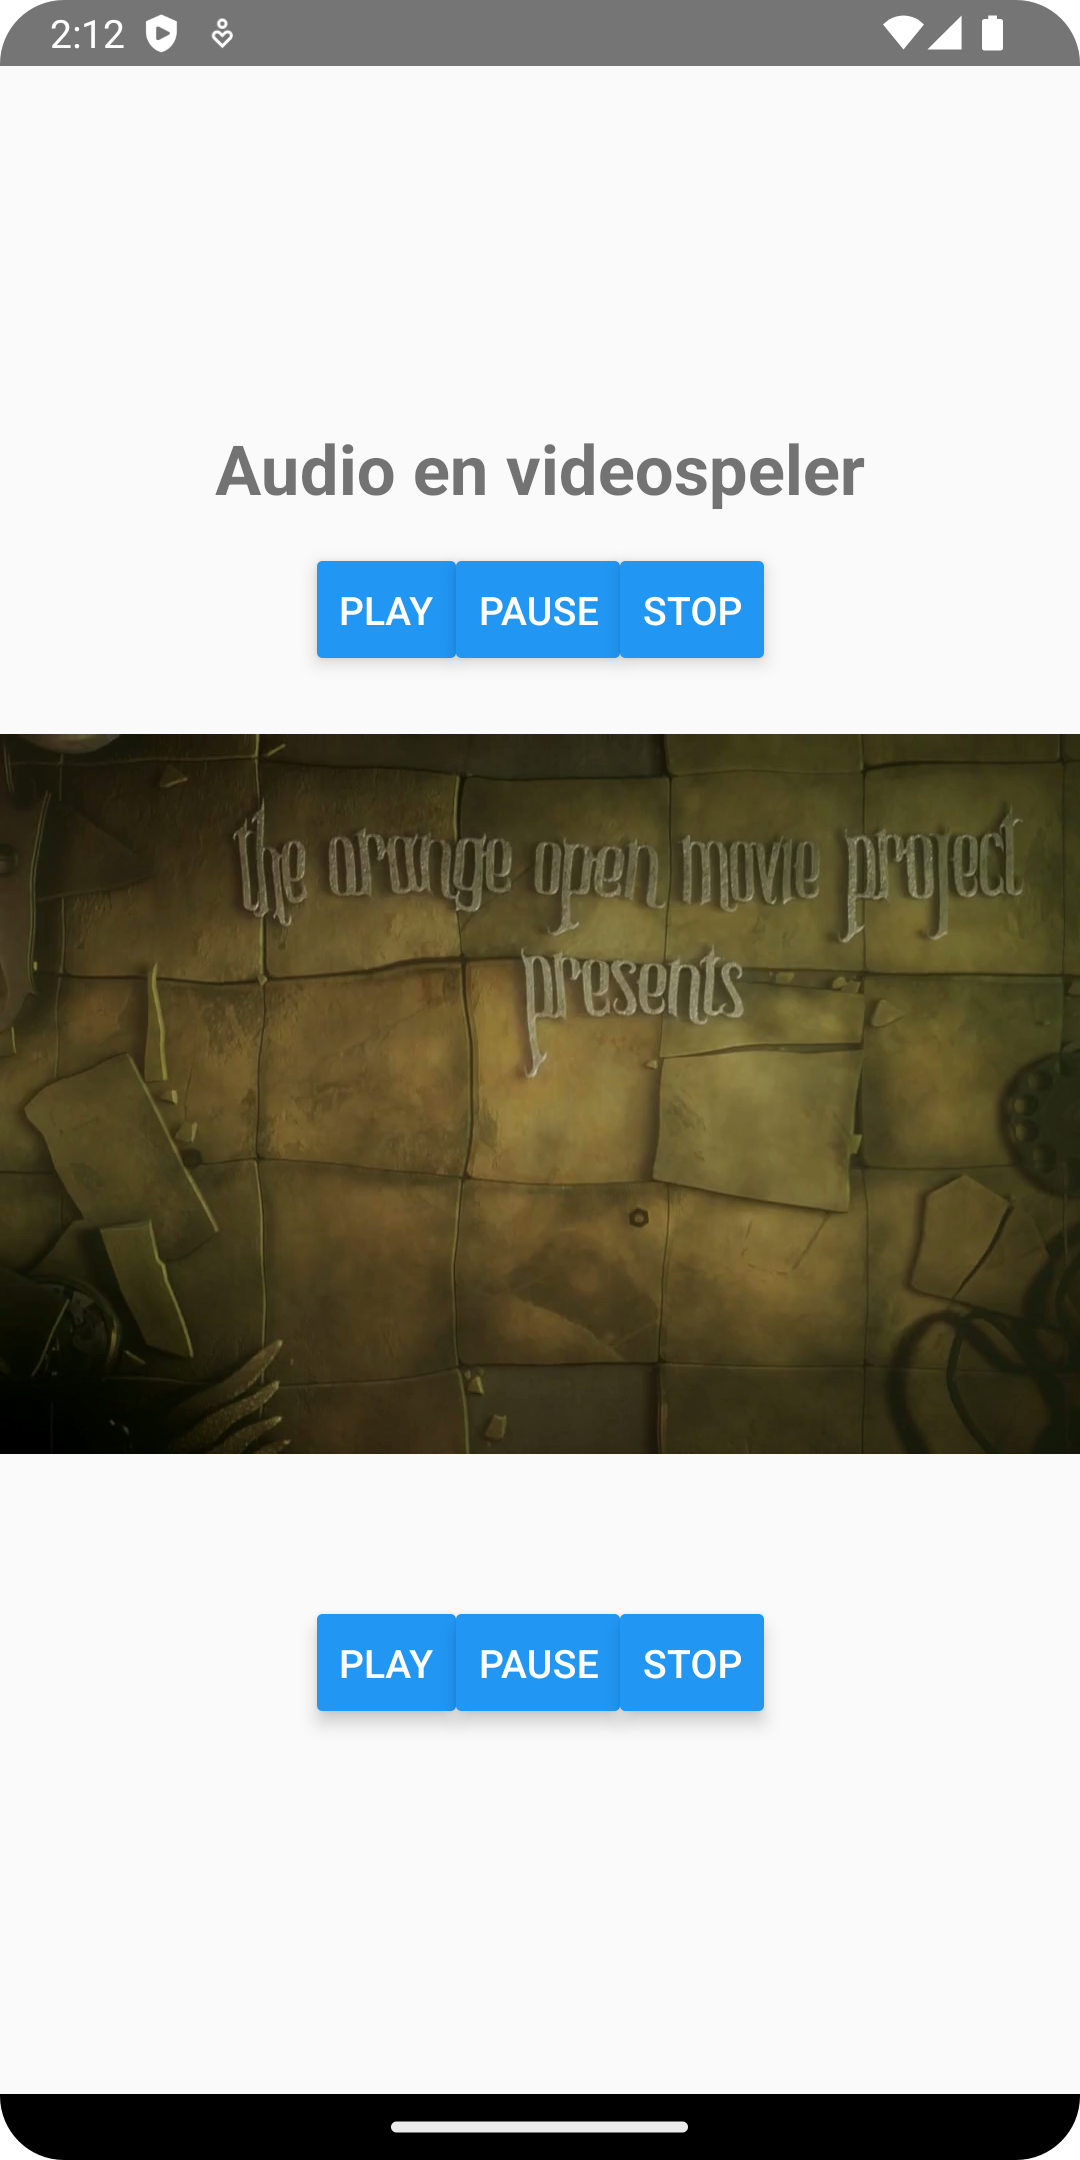
\includegraphics[height=0.4\textheight]{media_layoutcross.png}
    \caption{Layout van applicatie voor het afspelen van audio en video bij React Native.}
\end{figure}




\subsubsection{Ontwikkeltijd}

Aangezien dat de extra library react-native-track-player gebruikt wordt, wat een zeer 
uitgebreide library is en soms complex kan overkomen, is de ontwikkelingstijd hoger dan bij native. 
Ook moeten er meer stappen ondernomen worden om de TrackPlayer werkend te krijgen.
De extra complexiteit van react-native-track-player kan ook een voordeel zijn. Want indien de
extra functionaliteit van react-native-track-player nodig is, kunnen deze makkelijk geïmplementeerd worden.
Terwijl dit bij andere libraries of bij native niet altijd even makkelijk is.
\\\\
Voor videos af te spelen moesten we dan weer een andere library implementeren, wat ook weet 
tijd in beslag neemt. Maar deze library is wel makkelijk te implementeren en te gebruiken.
In totaal heeft het ongeveer 2 uur geduurd om de audio en video speler te implementeren.



\subsubsection{Performantie}

\paragraph{Tijdsduur}
Net zoals bij native wordt er enkel naar het CPU en geheugen gebruik tijdens 
het afspelen van audio en video gekeken.

\paragraph{CPU \& geheugen}
\begin{figure}[H]
    \centering
    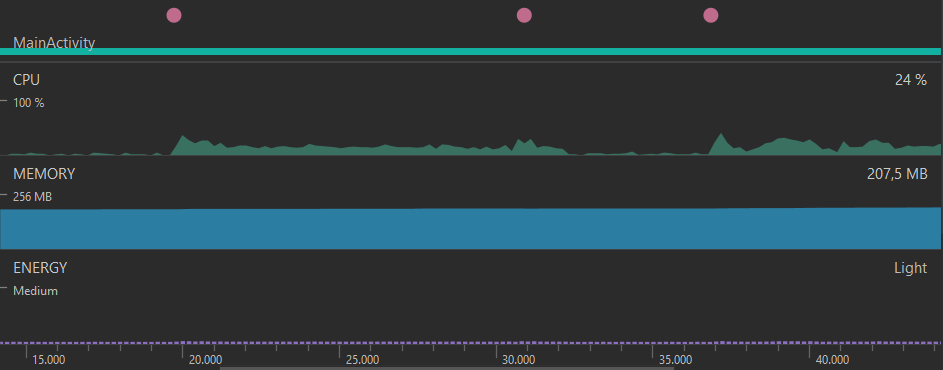
\includegraphics[height=0.25\textheight]{mediaPerformantieCross.png}
    \caption{Overzicht CPU en geheugen gebruik tijdens het afspelen van audio en video bij React Native.}
\end{figure}
Bij het eerste klik event voor het starten van de audio stijgt het
CPU gebruik tot 42\% en zakt daarna af tot een wisselend gebruik van 15 - 25\%. Bij het
tweede klik event voor het pauzeren van de audio stijgt het CPU gebruik tot 35\%. 
Bij het derde klik event voor het starten van de video stijgt het CPU gebruik tot 43\% en 
blijft dan schommelen tussen 10 - 35\%. Tijdens het afspelen van de audio en video blijft 
het geheugen gebruik rond de 207MB hangen. Er is dus geen verschil in
geheugen gebruik bij het afspelen van audio of video en het inactief zijn van de applicatie.


\subsubsection{Schaalbaarheid}

\paragraph{Complexiteit}
De gebruikte library react-native-track-player kan nogal complex overkomen. De library 
biedt heel wat mogelijkheden aan die niet altijd nodig zijn. Ook zijn er redelijk wat stappen 
nodig om de TrackPlayer werkend te krijgen. In sommige situaties kan 
react-native-sound of react-native-sound-player een betere keuze zijn maar in sommige gevallen kan 
de extra complexiteit van react-native-track-player ook een voordeel zijn. 

De gebruikte library react-native-video is gemakkelijk om te implementeren en te gebruiken.
Na het installeren van de library is er direct toegang tot de \textbf{<Video>} component
die dan gebruikt kan worden om video's af te spelen.

\paragraph{Herbruikbaarheid}
Het is mogelijk om alle functionaliteiten van bijvoorbeeld de audio- en videospeler elk in een 
aparte component te steken, zodat deze gemakkelijk op andere plaatsen in de applicatie kunnen worden 
gebruikt. Maar dit is niet altijd
nodig. In sommige gevallen is het ook mogelijk om de audio- en videospeler in één component
te steken. Dit is bijvoorbeeld het geval wanneer de audio- en videospeler eenzelfde functionaliteit
hebben. Desondanks is het wel mogelijk om de audio- en videospeler in aparte componenten te steken
en deze dan op meerdere plaatsen in de applicatie te gebruiken. Ook is het mogelijk om ze dan 
individueel op te schalen.



\section{Conclusie}
Bij het geheugen is te zien dat er geen verschil is tussen het afspelen van audio of video 
en het inactief zijn van de applicatie. Desondanks is het geheugengebruik bij cross-platform veel 
hoger dan bij native. Er wordt bij native maar 73MB gebruikt in vergelijking met 207MB 
bij cross-platform, een verschil van 183,56\%.
\\\\
Bij het CPU gebruik scoort native opnieuw beter dan cross-platform. Zowel bij het afspelen van audio als video 
is het CPU gebruik bij native lager. Bij het afspelen van audio bij 
native is de beginpiek 17\% en de eindpiek 23\%. Bij cross-platform is de 
beginpiek 42\% en de eindpiek 35\% terwijl het gemiddeld CPU gebruik bij native 0-1\% is en bij
cross-platform 20\%. Bij het afspelen van video bij native is de beginpiek 17\% en de eindpiek 16\%.
Bij cross-platform is de beginpiek 43\% en de eindpiek 28\% terwijl het gemiddeld CPU gebruik bij
native 4\% is en bij cross-platform 22\%. 
\\\\
\begin{tabular}{ |p{3cm}||p{5cm}|p{5cm}| }
    \hline
    \multicolumn{3}{|c|}{Audio} \\ 
    \hline
     & Native (Android) & Cross-platform (React Native) \\
    \hline
     & \multicolumn{2}{|c|}{Geheugen} \\ 
    \hline
    Offset & 2-3MB & 1-2MB \\
    Gemiddeld & 73MB & 207MB \\
    \hline
     & \multicolumn{2}{|c|}{CPU} \\
    \hline
    (Start)Piek & 17\% & 42\% \\
    (Eind)Piek & 23\% & 35\% \\
    Offset & / & 5\% \\
    Gemiddeld & 0-1\% & 20\% \\
    \hline
    \multicolumn{3}{|c|}{Video} \\ 
    \hline
     & Native (Android) & Cross-platform (React Native) \\
    \hline
     & \multicolumn{2}{|c|}{Geheugen} \\ 
    \hline
    Offset & 2-3MB & 1-2MB \\
    Gemiddeld & 73MB & 207MB \\
    \hline
     & \multicolumn{2}{|c|}{CPU} \\
    \hline
    (Start)Piek & 17\% & 43\% \\
    (Eind)Piek & 16\% & 28\% \\
    Offset & 3\% & 12\% \\
    Gemiddeld & 4\% & 22\% \\
    \hline
\end{tabular}
\\\\
De ontwikkeltijd bij
native ligt veel lager dan bij cross-platform. Dit komt omdat native gemakkelijker is om te implementeren en te gebruiken.
En omdat er geen extra libraries nodig zijn. Terwijl dit bij cross-platform wel het geval is.
Het kan echter de moeite waard zijn om extra tijd te investeren in cross-platform ontwikkeling 
aangezien de gebruikte bibliotheek extra functionaliteit biedt, zoals bijvoorbeeld de 
mogelijkheid om audio en video in de achtergrond af te spelen. Dit kan helpen bij eventuele 
uitbreidingen in de toekomst.
\\\\
Op basis van de verzamelde gegevens kan geconcludeerd worden dat voor het afspelen van audio en video native de beste keuze is.
Dit komt omdat native beter scoort op vlak van performantie. Ook is native gemakkelijker te implementeren
en te gebruiken. Daarnaast zijn er geen extra libraries nodig voor de implementatie. Let wel op, dit is enkel het geval
wanneer er geen extra functionaliteit nodig is. Indien er extra functionaliteit nodig is, kan
cross-platform een betere keuze zijn. Je zal in dat geval wel met een groot performantieverschil zitten.
















